\documentclass[12pt,parskip]{komatufte}\right 
\usepackage[subpreambles=false]{standalone}

%%%%%%%%%%%%%%%%%%%%%%%%%%%
% Silence warning messages
\usepackage{silence}
\WarningsOff[scrlayer-notecolumn]
\WarningsOff[biblatex]

%%%%%%%%%%%%%%%%%%%%
% Commenting

%\usepackage[author=Lyndon]{pdfcomment}
%\newcommand{\pdfcomment}[1]{} %ignore all comments

%\usepackage{todonotes}
%\newcommand{\pdfcomment}{\todo}


%%%%%%%%%%%%%%%%%%%%
% Tables
\usepackage{booktabs}

%%%%%%%%%%%%%%%%%%%
% Fonts
\usepackage{tgadventor} %sans
\usepackage{tgpagella}  %serif
\usepackage{inconsolata} %mono
\usepackage[T1]{fontenc}

\usepackage{microtype}
\usepackage[all]{nowidow}
%%%%%%%%%%%%%%%%%%%%%%%
% Styling
\setcounter{secnumdepth}{4}
\setcounter{tocdepth}{2}

\usepackage{placeins}



%%%%%%%%%%%%%%%%%%%
% Math
\usepackage{amsmath, amssymb, stmaryrd, mathtools}
\DeclareMathOperator*{\argmin}{argmin}
\DeclareMathOperator*{\argmax}{argmax}

\usepackage{xparse,xstring,etoolbox}
% crossref this against notation section
\newcommand{\vv}[1]{\tilde{#1}} % vector
\newcommand{\seq}[1]{\mathcal{#1}} % sequence
\newcommand{\set}[1]{\mathbb{#1}} % set

%%%%%%%%%
% Indexing/sequence indexing
\newcommand{\seqind}[2]{#1^{#2}} % seqence index
\newcommand{\ind}[2]{#1_{#2}} % indexed
\newcommand{\disamb}[2]{#1^{\mathrm{#2}}} %disambiguated

%% Smart indexing and naming
\newcommand{\ifupper}[3]{
    \normalexpandarg
	\exploregroups
	\StrCount{ABCDEFGHIJKLMNOPQRSTUVWXYZ}{#1}[\uppercount]
	\ifnumgreater{\uppercount}{0}{#2}{#3}
}

%smart index
\DeclareDocumentCommand{\ii}{u{_} m}{
	\ifupper{#1}%
	{% just a single uppercase character, i.e. a matrix
		  %make sure the index is the right length
		\StrCount{#2}{,}[\indcount]
		\ifnumgreater{\indcount}{0}
		{ % Got multiple indexes so all good
		 	\ind{#1}{#2}
		}
		{ % Only 1 index so grab the column
		 	\ind{#1}{{:,#2}}
		}
	}%
	{% Not just a single upper case character
		\ind{#1}{#2}
	}
}

\DeclareDocumentCommand{\nn}{u{_} m}{
	\seqind{#1}{#2}
}

\DeclareDocumentCommand{\dd}{u{_} m}{
	\disamb{#1}{#2}
}

% Index of a vector
\DeclareDocumentCommand{\iv}{u{_} m}{\ii{\vv #1}_{#2}}
\DeclareDocumentCommand{\dv}{u{_} m}{\dd{\vv #1}_{#2}}
\DeclareDocumentCommand{\nv}{u{_} m}{\nn{\vv #1}_{#2}}

%exp
\let\oldexp\exp
\renewcommand{\exp}[1]{\oldexp \left( #1 \right)}
\newcommand{\exptwo}[1]{\oldexp_2 \left( #1 \right)}

\newcommand{\softmax}{\mathrm{smax}}

\DeclareMathOperator*{\expectedop}{\mathbb{E}}
\DeclareDocumentCommand{\expected}{u{_} m}{
	\expectedop\limits_{\mathrlap{#2}}
}

%%%%%%%%%%%%%%%%
%Graphics
\usepackage{tikz}
\usetikzlibrary{positioning, fit,  shapes.geometric}
\usepackage{ifthen}
\usepackage{etoolbox}

\tikzset{
	backgroundcolor/.style ={fill=white},
	every node/.append style={
		minimum height=7mm,
	},
	labe/.append style={
		%Blue,
		align = center,
		backgroundcolor,
		fill opacity=0.6,
		text opacity=1,
		font={\footnotesize\itshape}	
	},
	layer/.append style={
		draw,
		align = center,
		minimum height=7mm,
	},
	tight/.append style={
		inner sep=0.2mm,
	},
	lookupbox/.append style={
		draw=none,
		append after command={
		       	[shorten <= -0.5\pgflinewidth]
		       	([shift={(-1.5\pgflinewidth,-0.5\pgflinewidth)}]\tikzlastnode.north east)
		       	edge([shift={( 0.5\pgflinewidth,-0.5\pgflinewidth)}]\tikzlastnode.north west) 
		       	([shift={( 0.5\pgflinewidth,-0.5\pgflinewidth)}]\tikzlastnode.north west)
		       	edge([shift={( 0.5\pgflinewidth,-1.5\pgflinewidth)}]\tikzlastnode.south west)            
		       	([shift={( -1.5\pgflinewidth,+0.5\pgflinewidth)}]\tikzlastnode.south east)
		       	edge([shift={(-1.5\pgflinewidth,-0.5\pgflinewidth)}]\tikzlastnode.north east)
		},
		inner sep=0.7mm,
		outer sep=0mm,
		minimum width=25mm
	}
}

\usepackage{pgfplots}
\pgfplotsset{compat=1.14}
\pgfplotsset{sideplot/.append style={
		width=\notescolwidth,
		domain=-10:10,
		samples=101,
		smooth,
		enlarge y limits={abs=2},
		axis lines=middle,
		xlabel  = $z$,
		ylabel  = $y$,
	},
	equ/.append style={
		color=blue,
		thick,
		mark=none
	}
}

% Function  For a plot 
% it  needs to be declared in preamble because of how \makenote* interacts with multiple files
\def\errorsurface(#1,#2){(0.5*#1 + 0.7*#2 + sin(deg(1.5*#1 + #2^2)))^2}


\usepackage{graphicx}
\graphicspath{{./figs/}, {./}, {./figs/chaptersentencerrepr/}, {./figs/chapterintromachinelearning/}, {./figs/chapterwordrepr/}}
\usepackage{adjustbox}


%%%%%%%%%%%%%%%%%%%
% Refs
\usepackage{cleveref}

\addbibresource{master.bib}

%%%%%%%%%%%%%%%%%%%%
% Formatting

% for examples from natural language space.
\newcommand{\natlang}[1]{\ifmmode \text{``\texttt{#1}''} \else {``\texttt{#1}''}\fi}
% \ifmmode ``trick'' from https://tex.stackexchange.com/a/15194/5834

%%%%%%%%%%%%%%%%%%%%%


\begin{document}
	

\setchapterpreamble{%
	\dictum[J. M. G. ele Lammens, PhD Dissertation,
	\textit{A~Computational Model of Color Perception and Color Naming},  State University of New York, 1994]{%
Whether one sees the artificial neural network technique described below as learning or as optimization depends largely on one's background and one's theoretical likes and dislikes. I will freely use ``learning'' in the remainder of this section because that term is traditionally used in the neural networks literature, but the reader should feel free to substitute ``optimization'' if (s)he finds the other term offensive. Please contact the author for an Emacs lisp function to enforce the usage of choice.%
}}
\chapter{Introduction to neural networks for machine learning}\label{sec:machine-learning-for-representations}
\aside[Suggested Reading]{ As this is not a comprehensive introduction we recommend the reader look elsewhere for additional reading.
In particular we recommend
the free online web-book: \citetitle{WebBookBackprop} \parencite{WebBookBackprop},
and the comprehensive: \citetitle{TheDeepLearningBook} \parencite{TheDeepLearningBook}
}

\pdfcomment{Should recommend 3 or so books. but I only know that one as being really good}

\begin{abstract}
	This chapter covers the crucial machine learning techniques required to understand the remained of the book: namely neural networks.
	Readers already familiar with neural networks can freely skip over this chapter.
	It does not cover all aspects of machine learning, or even neural networks, which would be many entire books on their their own.
	A large portion of this section is dedicated to recurrent neural networks, and these are very important in natural language tasks.
\end{abstract}

Machine learning, particularly neural networks has become a hot topic of late.


The core notion of machine learning is to learn a to perform an function based on examples.
This is in-contrast to ``regular programming'' where code is written to accomplish the function based on the programmer's analysis of the task.
Machine learning is at its most useful when it is difficult to articulate explicit rules for finding an output for an input; but for which there are many examples of such.
For example, the rule of English spelling ``I before E, except after C'', is known to be often incorrect.
It is hard to write a rule about letter order.
However, a dictionary (or any other corpus) will have thousands of words showing the correct order.
By applying suitable machine learning techniques,
a system could learn to determine the correct spelling of words containing \natlang{ie} and \natlang{ei},
and inform the users as to if an input word is correct, even if the word never occurred in the training dictionary.
This is because the machine learning algorithm (ideally) discovers generalisable rules, from the training examples.
For most machine learning methods, including neural networks, these rules are not in a readily interpretable form, but are stored as numerical parameters of the model.

\section{Neural Networks}
\aside[Multilayer perceptron or Artificial Neural Network?]{An artificial neural network is sometimes called a multilayer perceptron.
This is in reference to the related perceptron learning algorithm.
This term has fallen out of favour in newer works,
with Hinton, who originally coined the term, expressing his own regret at the naming.
However, in any case they refer to the same thing.
}

A neural network is one particular family of machine learning algorithms.
It is important to understand that neural networks are not emulations of the brain,
they are algorithms that were inspired by the ideas about how the brain worked \pcite{hebb1949organization}.
Some advancements have also been inspired by the functioning of the brain,
but many others have come from statistical methods or elsewhere.
A neural network is no more similar to a brain, than it is to a Fourier transform.

The core idea behind a neural network is to represent the transformation of the input to the output as links between neurons in a sequence of layers.
Each neuron has a weighted connection the the neurons in the layer below,
and it applies a nonlinear function to this weighted sum, 
to determine its own output.
The output is connected to the inputs in the layer above, or is the final output.

\pdfcomment{Maybe a diagram and/or some equations here. and a bit more detail?}


\aside[Don't implement neurons]{
Typical object orientated programming teaches one to look for objects.
A obvious object in a neural network would be a neuron.
Another object could be the connection (weight).
Perhaps a different subclass of neuron for each activation function.
Don't do this.
It will be incredibly slow in almost any programming languages -- where objects are always stored by reference, thus requiring a pointer dereferencing for each operation on each neuron.
Object orientated is not a good paradigm for this kind of technical computing.
Instead program in terms of matrix's and vectors.
Potentially using objects for layers.
This allows one to take advantage of efficient matrix algrabra routines such as in BLAS and LAPACK.
}



\section{Function Approximation}

The universal approximation theorem (UAT) tells us that a neural network can be used to approximate almost any function \parencite{mhaskar1992uat,leshno1993uat,SONODA2017uat}.
Here a function should be understood in the general sense -- classification is a function from observations to classes, regression is a function from observed values to target values.
More precisely, for any continuous bounded function,
the UAT states that there there exists a neural network that can approximate that function, to any given degree of accuracy.
Further, it states that the network only needs a single hidden layer.
In a less rigorous sense, of approximation, such a continuous bounded function can approximate any function, over a restricted sub-domain of input values.

The earliest proofs of this was restricted to bounded activation functions like the sigmoid .
More recent work has extended this for unbounded activation functions like ReLU \pcite{SONODA2017uat}.

A network without any hidden layers is only able to approximate linear functions.
It is equivalent to a perceptron, or a linear SVM. 


However, the UAT does not tell us the values for those weight parameters,
nor does it promise that any method of training will ever reach them in finite time.
More significantly it does not inform as to how wide \emph{sufficiently wide} is,
nor if deeper is more efficient than wider.


\section{Network Hyper-parameters}
\aside[Hyper-parameters vs Parameters]{
	The weights and biases of the network are called its parameters.
	They are optimised during training.
	The other features of the network, including its topology, activation functions, and the training method (which often has its own set of options), are called the hyper-parameters. 
}

The key determination in applying neural networks to any problem,
is the choice of the hyper-parameters.
Including, the number of hidden layers, and their widths.
Neural networks can largely be thought-off as black-boxes,
that can be trained to  accomplish tasks given a set of training examples.
Beyond recognising how to express the problem,
the chose of hyper-parameters is the most important decision when employing a neural network based solution.


\subsection{Width and Depth}
While the UAT has shown that a single hidden layer is sufficient,
it is not necessary optimal in terms of achieving best performance in practice.
For many problems it is better to have a deeper rather than wider network.
This realisation and the techniques to overcome issues relating to deeper networks has lead the current deep learning trend.

In the last decade, deep nets have come back into fashion.
In brief the reasoning for this is a combination of a better techniques (e.g. ReLU, unsupervised pretraining),
better hardware (e.g. GPUs and Xeon Phi), and more labelled data (e.g. from crowd-sourcing platforms such as Amazon Mechanical Turk.)
This has allowed problems that were previously considered unsolvable with earlier shallow networks to be solved with deep networks achieving state of the art results.

\aside[What happened to Deep Belief Network Pretraining?]{
	\textcite{hinton2006fastDBN,bengio2007greedylayerwise} lead to a new resurgence of interest in neural networks.
	Pretraining with Deep Belief Networks allowed for deep networks to be trained.
	It was held for many years that it was necessary to use layer-wise unsupervised pretraining,
	even when one has only supervised data. 
	\textcite{glorot2011deepRELUsparse} showed that with ReLU units, a deep network could be trained directly and achieve the same performance.
	As such unsupervised pretraining is now a more niche technique used primarily when there is an excess of unsupervised data.
}

The choice of the number of hidden layers (depth),
and the sizes (width) is a key parameter in designing a neural network.
It is arguably \emph{the} key parameter.
It can be assessed using a hyper-parameter sweep on a validation or development dataset.
It is a particularly relevant parameter for our purposes, as hidden layers normally are directly linked to our representations of natural language.



\subsection{Activation functions}

\aside[Notation: Generic Activation Function $\varphi$:]{Though-out this book, when the activation function is not significant to the problem at hand, we will represent it with the \mbox{symbol $\varphi(\cdot)$.}}

The universal approximation theorem places a number of requirements on the activation function.
These requirements have been progressively relaxed by works such as \textcite{leshno1993uat, SONODA2017uat}.
This section discusses a number that are in common use today.

The choice of activation function determined the range of output of a neuron.
For the hidden layers these generally perform relatively similarly.
Sigmoid, tanh, and ReLU are the most common activation functions used for hidden layers.
The range of output of a hidden layer does not normally matter, as it is by definition hidden.
More significantly, the final activation function or the output function does always matter.
The output function should be chosen for the task at hand.
As will be discussed in \Cref{sec:rnn} this also has significance when designing gating neural network structures.

Beyond determining the range of the output, its derivative also determines the behaviour during training via gradient descent based training methods.
This is significant for activation functions like ReLU and ReLU6 discussed below.


In the following sections $y$ is the vector output from this layer, and $z$ is its input.

\subsubsection{Linear/Affine}
A linear or affine layer is the most basic activation function.
Arguably not truly an activation function at all, the true activation function associated with it would be the identity function.
It is commonly used as an output function for regression tasks.
\begin{equation}
y=Wz + b
\end{equation}
In this equation $W$ and $b$ are a trained matrix and vector respectively.
This allows the output to be any value, within some set of bounds learned during training.
However, when this is not needed it increases the difficulty of training for no benefit.

It is normal to have such a transform on every layer.
This defined the layers as fully connected.
As it allows the scaling and shifting of any of the other activation functions.


Linear layers, cannot on their own, be used as hidden layer activation functions.
A stack of linear layers simplifies to be equivalent to a single linear layer, which means that the network can only approximate linear functions.
A non-linearity is required.
This is what the other activation functions provide.


\subsubsection{Sigmoid}

\asidefig[The sigmoid function]{
\begin{tikzpicture}
\begin{axis}[sideplot, enlargelimits={rel=0.25}]
\addplot+[equ] {1/(1+exp(-x))};
\end{axis}
\end{tikzpicture}
}

This is the classic neural network activation function.
\begin{equation}
y=\sigma(z)=\frac{1}{1+e^{-z}}
\end{equation}
Sigmoid output values are between zero and one.
If the network has a single output then this is a fuzzy boolean.
It can be used to classify into two categories.
It is sometimes called a logistic output function.

\subsubsection{Softmax}
\aside[multinomial logistic regression]{A neural network classifier with a softmax output layer is sometimes called a multinomial logistic regression network (especially if there is no hidden layer).
	This can lead to some confusion with a sigmoid outputting network.
	However, the similarity can be understood by considering a softmax output layer with 2 classes.
	This reduces to $s_m(z)= \left[ \sigma(z), 1-\sigma(z) \right]$.
}

Softmax is the standard output layer for categorical classification.
Formally, one should say that it is a regression to a class probability, rather than a true classifier as it does not return the class.
We will use the terms interchangeably.

For $y_i$ being the $i$th output, which gives the probability of being in class $i$.
\begin{equation}
y_i=\left(s_m(z)\right)_i=\left( \frac{e^{z_i}}{\sum_{j=1}^{j=N} e^{z_j}} \right)
\end{equation}
For $N$ the number of outputs equal to the number of categories in the classification.

These outputs have  values are between zero and one, and sum to one.
They thus define a discrete, probability mass function (pmf).

Softmax is a \emph{soft}, i.e. differentiable,  version of what could be called \emph{hard-max}.
In this conceptual hard-max function, the largest output is set to one, and the others set to zero.
It is non-differentiable and thus not suitable for use in a neural network.
In softmax the largest values is proportionally increased to be closest to one,
and the smallest to be closest to zero.

Further consideration of the softmax is given in \Cref{sec:softmax-and-bayes-theorem}.

\subsubsection{Tanh}
\asidefig[the tanh function]{
	\begin{tikzpicture}
	\begin{axis}[sideplot, enlargelimits={rel=0.25}]
	\addplot+[equ] {tanh(x)};
	\end{axis}
	\end{tikzpicture}
}

The hyperbolic tangent function is a  scaled and shifted sigmoid function.

\begin{equation}
y=\tanh(z)=\frac{e^{2z}-1}{e^{2z}+1}=2\sigma(2z)+1
\end{equation}

The notable difference is that outputs are restricted to be between $-1$ and $+1$.

\subsubsection{ReLU}
\asidefig[The ReLU function]{
	\begin{tikzpicture}
	\begin{axis}[sideplot, enlarge y limits={abs=2}, enlarge x limits={abs=0.25}]
	\addplot+[equ] {max(0,x)};
	\end{axis}
	\end{tikzpicture}
}

The Rectified Linear Unit (ReLU) is a more recently popularized activation function \pcite{dahl2013reludropout}.
It comes from earlier neuroscience work \pcite{hahnloser1998piecewise}.
\begin{equation}
y=ReLU(z)=\max \left( 0, z \right)=\begin{cases}
z & 0\le z\\
0 & z<0
\end{cases}
\end{equation}
Values are restricted to be at non-negative.
As this function has derivative zero for $z<0$, once a unit is turned off, it is not turned back-on.
As during gradient descent the derivative to modify weights in its inputs will always be zero.
This is commonly called the neuron dying.
Further to this, using random initialization this ensures that half of all neurons in the layer will be never turned on.
Thus resulting in sparse connections between the layers.
This has been found to be a good thing \pcite{glorot2011deepRELUsparse}.
ReLU is very commonly used as a hidden layer activation function for deep networks.
It also helps with the gradient vanishing and gradient exploding problems that occur in deep networks.
\pdfcomment{I think maybe this whole section needs to be moved to after I have explained gradient descent?}


\subsubsection{RELU6}
\asidefig[The RELU6 function]{
\begin{tikzpicture}
\begin{axis}[sideplot,  xtick={-6,-3, 0,3,6}, ytick={-3, 0,3,6}, enlarge y limits={abs=2}]
\addplot[equ] {max(0,min(x,6))};
\end{axis}
\end{tikzpicture}
}


Closely related to ReLU is ReLU6 \pcite{krizhevsky2010convolutional}.
This is another linear unit the saturates at 0, but also at 6.
\begin{equation}
y=ReLU6(z)=\max \left(0, \min\left(6, z\right) \right) =  \begin{cases}
6 & 6<z\\
z & 0\le z\le6\\
0 & z<0
\end{cases}
\end{equation}
\aside[Why are we bringing up ReLU6?]{ReLU6 is one of the more obscure activation functions. As such it may seem a bizarre inclusion in this shorter introduction. However, we have found it surprisingly successful as an activation function, e.g. in the auto-encoder example which follows in \Cref{sec:bottle-necking-autoencoder}.}

This has similar advantages to ReLU.
However, as well as units being able to die to zero, it can also die to positive.
The bounding at 6, rather than any other number is rather arbitrary -- particularly given scaling with the intervening affine layers.
The important point is that it is bound both above and below.
Unlike ReLU, it fully meets the requirements for the original UAT, which is nice for proving theoretical capabilities of variant networks as it hugely simplifies the proofs.



\subsubsection{Other activation functions}

There are numerous other activation functions.
Most are of interest for use in hidden layers such as Leaky RELU, Softplus, ELU and many others.
For specialized tasks, other functions might be used, such as atan2 \pcite{WhiteRepresentingAnglesSE}.


\section{Training}
The process of training the network is the process of solving a very high dimensional, nonlinear, non-convex global optimization problem.

\aside[Evaluation function vs Loss function]{
	We must distinguished between two types of \emph{error function}.
	The \emph{evaluation function} is the metric we are truly trying to improve, this could be accuracy for classification, BLEU score for translation, F1 score for retrieval etc.
	It is applied to the whole system (which may be greater than just the neural network), and the system may be evaluated in different ways using different evaluations.
	As the evaluation is often not differentiable, a proxy for it which we call the \textbf{loss function} is used in training.
	For example, squared error for regression, or cross-entropy for classification.
	The loss function is applied to the output of the network during training to calculate the error between the network output for a given input, and the target output from the training example.
	The loss function is such that minimising the loss function also (ideally) results in the true evaluation function being optimised.
}

Finding the globally optimal solution to such a problem would is a very difficult problem.
Nonlinear and non-convex problems can have local minima that are not global minima.
This means they can not be guaranteed to be solved  a global optima by gradient descent.
However, this does not pose an issue for more neural networks as finding the true global optima is not required, merely finding a \emph{good enough} set of weights to get a \emph{good enough} result.

To train the network one must find the values for the networks weight and bias parameters, such that that total loss function is minimized over the training set.

To define the training problems as an optimisation problem one first considers the loss function for a single training case.
For a target outputs $y$ and an actual outputs $\hat{y}$, a loss function is defined $loss(y, \hat{y})$.
For example the squared error loss (sometimes called L2 loss) used in regression is defined by 
$SE(y, \hat{y})=\sum_{\forall i} (y_i-\hat{y_i})^2$.
The cross-entropy loss used in binary classification is defined by
$CE(y, \hat{y})=-\sum_{\forall i} (1-y)(\log (1-\hat{y}))) + y(\log (\hat{y})))$.
The choice of loss function depends on the purpose of the network.

The network function is composed into the loss function.
to the per training case loss, for a training case loss: $loss(y, N(x,\tilde{P}))$.
For $N(x,\tilde{P})$ being the function that executes some neural network, with weight and bias parameters all grouped into given by $\tilde{P}$, upon an input $x$ where the target output is $y$ and the actual output is $\hat{y}$.

The total loss is defined by taking the mean over the whole training set batch ($\mathcal{X}$):
\begin{equation}
loss_{total}(\tilde{P}) = \frac{1}{|\mathcal{X}|}\sum_{\forall (x, y)\in\mathcal{X}} loss(y, N(x),\tilde{P}))
\end{equation}
This is now nothing but a nonlinear function to be minimised by adjusting the values of the weights and biases in $\tilde{P}$.


This can be given to off-the-shelf  unconstrained nonlinear optimisation algorithms \pcite{Ngiam2011} such as L-BFGS  \parencite{nocedal1980updating}.
Alternatively, and more commonly, the loss and updated can be processed iteratively on sub-sets (minibatches) of the training data at a time -- often using optimisation algorithms specifically targeted at machine learning applications such as Adam \parencite{kingma2014adam}.
In either case, almost all optimizers used for neural networks rely on gradient descent.

\aside[AdaGrad, AdaDelta, and Adam]{
AdaGrad \parencite{AdaGrad}, AdaDelta \parencite{DBLP:journals/corr/abs-1212-5701} and Adam \parencite{kingma2014adam}
 are effectively successive iterations of an optimisation algorithm specifically targeted at the machine learning case.
In these algorithms dynamically adapt the learning rate during training.
There are several other algorithms in the family.
In recent works, Adam is the most commonly used optimiser.
We suggest there is an interesting theoretical space about the relationship between adapting the learning rate, and implicitly finding the second derivative as in the more traditional quasi-Newtonian methods.}


\subsubsection{Gradient Descent and Back-propagation}
\aside[Back-propagation vs Gradient Descent?]{%
	Formally speaking, back-propagation finds the gradients, and Gradient Descent uses those gradients to update the network parameters.
	However the two terms of often used interchangeably.
}


Gradient descent is, as mentioned, the basis of most commonly used optimisers in machine learning.
In gradient descent based methods the derivative of the loss function relative to the parameters are used to update the parameters.
The parameters in this case are the network weights and biases.
To calculate the gradients the back-propagation algorithm is used.

Back-propagation is simply a method of applying the well-known chain-rule of calculus to the neural network loss functions \pcite{backprop}.
It one to calculate:  $\frac{\partial loss_{total}}{\partial{W_{i,j}}}$
for any weight (or bias) parameter $W_{i,j}$ in the network.
These can always be found as the overall loss function, including the network, is differentiable \footnote{Technically most networks are differentiable almost everywhere. For some functions like ReLU they have some single points of where the derivative is not defined. But the derivatives here can be forced to a known value.} (when using typical activation functions and loss functions).

Using this gradient the network parameters can thus be updated.
Updating the parameters to a new value in the direction of the gradient decreases the loss (for the right step size).
This means for each $W_{i,j} \in \tilde{P}$ updating its value according to the local gradient.
\begin{equation}
W_{i,j} \leftarrow W_{i,j} - \alpha \frac{\partial loss_{total}}{\partial{W_{i,j}}}
\end{equation}
Where $\alpha$ is a update step size, commonly called the learning rate.
The more advance methods discussed earlier, such as Adam, and L-BFGS, are advancements on this same core principle.


If one considers a plot with the loss given on the vertical axis,
and the values of the parameters as describing a position on the horizontal axes,
then gradient descent is moving that the parameter-point downward on that surface based on local estimate of the slope.
\pdfcomment{Insert Plot Here}






\section{Some Examples of Common Neural Network Architectures}
\aside[These examples are available online]{For a practical introduction to the networks discussed here, worked examples of these network are available in the accompanying blog post at \url{http://white.ucc.asn.au/NNforNLPBook/NNexamples}.
	They are written in are in the Julia programming language, making use of the TensorFlow.jl package.
}

We will discuss more linguistically relevant neural networks in the following chapters.
However, to introduce the topic, we will give some basic examples.


\subsection{Classifier}\label{sec:classifier}
\aside[FashionMNIST]{is a new image classification benchmarking dataset \parencite{xiao2017/online}.
It is a task to classify images of shirts, shoes and bags etc.
It is an exact drop-in replacement for MNIST.
It was created to allow the same brenchmarking scripts to be used;
while using a different data set.
This combats extremely high use of MNIST leading to implicit test set information leakage in the design of ML systems;
as well as being a more difficult task, thus allowing better discrimination between systems.
}

A classifier on the MNIST challenge is one of the most common introductory networks.
The MNIST dataset is a collection of images of hand written digits, which much be classified as to which digit they are.

A basic network to complete this task is is shown in \Cref{fig:mnistnetwork}.

\begin{figure}
	\caption{The structure of a simple classifier network for MNIST.}
	\label{fig:mnistnetwork}
	\documentclass{standalone}

\usepackage{tikz}
\usetikzlibrary{positioning, fit,  shapes.geometric}
\usepackage{ifthen}
\usepackage{etoolbox}

\tikzset{
	backgroundcolor/.style ={fill=white},
	every node/.append style={
		minimum height=7mm,
	},
	labe/.append style={
		%Blue,
		align = center,
		backgroundcolor,
		fill opacity=0.6,
		text opacity=1,
		font={\footnotesize\itshape}	
	},
	layer/.append style={
		draw,
		align = center,
		minimum height=7mm,
	},
	tight/.append style={
		inner sep=0.2mm,
	},
	lookupbox/.append style={
		draw=none,
		append after command={
		       	[shorten <= -0.5\pgflinewidth]
		       	([shift={(-1.5\pgflinewidth,-0.5\pgflinewidth)}]\tikzlastnode.north east)
		       	edge([shift={( 0.5\pgflinewidth,-0.5\pgflinewidth)}]\tikzlastnode.north west) 
		       	([shift={( 0.5\pgflinewidth,-0.5\pgflinewidth)}]\tikzlastnode.north west)
		       	edge([shift={( 0.5\pgflinewidth,-1.5\pgflinewidth)}]\tikzlastnode.south west)            
		       	([shift={( -1.5\pgflinewidth,+0.5\pgflinewidth)}]\tikzlastnode.south east)
		       	edge([shift={(-1.5\pgflinewidth,-0.5\pgflinewidth)}]\tikzlastnode.north east)
		},
		inner sep=0.7mm,
		outer sep=0mm,
		minimum width=25mm
	}
}

\begin{document}

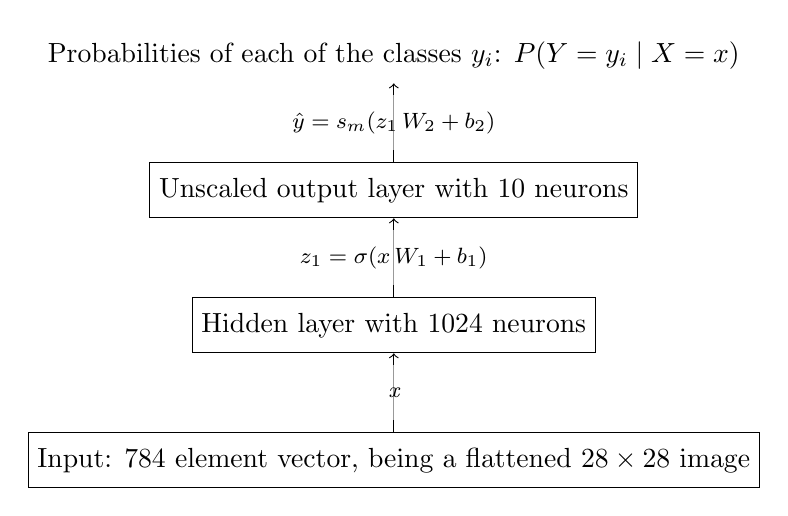
\begin{tikzpicture}[]

\node(in)[layer]{Input: 784 element vector, being a flattened $28 \times 28$ image};

\node(l1)[layer, above=of in]{Hidden layer with 1024 neurons};
\node(l2)[layer, above=of l1]{Unscaled output layer with 10 neurons};
\node(out)[above=of l2]{Probabilities of each of the classes $y_i$: $P(Y = y_i \mid X=x)$};

\draw[->] (in) edge  node[labe]{x} (l1);
\draw[->] (l1) edge  node[labe]{$z_1=\sigma(x\,W_1+b_1)$} (l2);
\draw[->] (l2) edge  node[labe]{$\hat{y}=s_m(z_1\,W_2+b_2)$} (out);

\end{tikzpicture}

\end{document}
\end{figure}

The network is defined by the equations:
\begin{align}
z=\varphi(W_1 x+b_1) \\
\hat{y}=s_m(W_2 z + b_2) \\
P(Y=i\mid X=x) &= \hat{y}_i \\
&= \left[s_m(b_2 + W_2 \varphi(b_1 + W_1 x))\right]_i
\end{align}
For $X$ the input variable of grey-scale pixels intensities, and $Y$ the output as a class.
The output is represented with 1 hot encoding, where the index corresponding to the class is 1, and the others zero.


\aside[This simple network performs very well]{
	We note that this simple network can without further enhancement exceed the early published results for the MNIST challenge, using standard un-augmented neural networks,
	simply by using a very wide hidden-layer, that was not feasible at the time of those benchmarks.
	It is still outperformed by convolution neural networks and other better architectures.
}

To go into details about each layer:
The input is given by the grey scale pixel indentities in the original $28\times 28$ image.
This is flattened giving a $784$ element sized vector ($x$).
The first weight matrix projects that up onto a hidden layer  of width $1024$.
Thus $W_1$ is a $1024\times 784$ matrix.
The bias $b_1$ is for that hidden layer, so it is a vector of length $1024$.
The hidden layer's actual activation values ($z$) for any input can be considered as being the values taken by 1024 different latent variables describing that input.
Variables that are chosen (via training) to be useful in discriminating the correct class for the next layer.

As this is a shallow network, without one hidden layer, the next layer is the output layer.
A deep network would have more hidden layers, for additional latent variables describing relations.
For the output layer we must project down to 10 dimensions, as there are 10 classes to choose from: the numbers from 0 to 9.
thus $W_2$ is a $10 \times 1024$ matrix,
and the bias $b_2$ is a 10 element vector.
Using the softmax layer here ensures that output $\hat{y}$ is a valid probability mass function (nonnegative and summing to one).


\subsubsection{Softmax and Bayes' Theorem}\label{sec:softmax-and-bayes-theorem}
As a digression, it is worth considering the similarity between a network with a softmax output layer, and the application of Bayes' Theorem.
This will become important for understanding output embeddings, and hierarchical softmax in the future chapters.

The conditional probability of a classification given the value of some observed variable is defined by $P(Y=y\mid Z=z)$.
For $Y$ being the class taking value $i$;
and $Z$ being the variable being conditioned upon, taking value $z$.
Here $z$  is some features vector, this could be the output of a hidden layer below, or it could be a direct input.
Using softmax the estimated probability is given by
\pdfcomment{It is probably needful to change y into i for index}
\begin{align} 
P(Y=i\mid Z=z)&=\frac{e^{[Wz+b]_{i}}}{\sum_{\forall j}e^{[Wz+b]_{j}}}
&=\frac{e^{[Wz]_{i}}\,e^{b_{i}}}{\sum_{\forall j}e^{[Wz]_{j}}\,e^{b_{j}}}
\end{align}

One can see that the bias term $e^{b_{i}}$ does not depend on the value of $z$.
The bias term is analogous to the prior probability. Literally, it is the bias towards each element (i.e. each value $Y$ could take) without observing the condition.
Marginalising the probability over all $Z$ values gives $P(Y=i)=e^{b_{i}}$. \pdfcomment{Shouldn't there be a denominator here?}

\pdfcomment{Is this actually a probability, or is it a score?}

The other component is $e^{[Wz]_{i}}$.
The key term here is $[Wz]_{i}$, by considering this for each index $i$ (class value) that $Y$ might take then
we have 
\begin{equation}
[Wz]_{i}=\sum_{\forall j}W_{j,i}\,z_{j}=W_{i}^{T}z.
\end{equation}
\pdfcomment{Check columns vs rows}.

Given one is considering the case for a particular $Y=i$, then 
it can be seen that the row vector $W_{i}^{T}$ as a weighting map for features possessed by $z$.

i.e for some scoring function $R$:
\pdfcomment{Is this actually a posterior probability, or is it just a score?}
\begin{equation}
R(Z=z\mid Y=i)=e^{[Wz]_{i}}
\end{equation}
which is very similar to a posterior probability.


Then reformulating the original statement we have:
\begin{equation}
P(Y=y\mid Z=z)=\frac{R(Z=z\mid Y=y)\,P(Y=y)}{\sum_{\forall i}R(Z=z\mid Y=i)\,P(Y=i)}
\end{equation}

Contrast this to Bayes' Theorem:
\begin{equation}
P(Y=y\mid Z=z)=\frac{P(Z=z\mid Y=y)\,P(Y=y)}{\sum_{\forall i}P(Z=z\mid Y=i)\,P(Y=i)}
\end{equation}

The similarities can be seen.
The bias effectively determines a prior probability like term.
The weights defines the posterior probability: that is the chance of a particular class having a particular set of features.
The rows of the weight matrix mark how important each hidden feature is to each class. \pdfcomment{check rows vs cols}
We can this consider that each row of the weight matrix is itself a representation itself of the class, as characterised by the importance of those latent features.
In the next chapter we will consider this as an output embedding.

A more traditional way of finding a representation of an input (rather than an output class) is to use an autoencoder.

\subsection{Bottlenecking Autoencoder}\label{sec:bottle-necking-autoencoder}
\begin{figure}
	\caption{A sampling of MNIST images from the test-set, arranged according to the values of 2 neurons on the encoding layer.}
	\label{mnist-encoding}
	\includegraphics[width=\textwidth]{figs/chapterintromachinelearning/mnist-encoding.png}
\end{figure}
An autoencoder is a tool primarily used for finding a representation of their input.
There are many varieties of autoencoder based on neural network related techniques, including the works of \textcite{hinton2002RBM,hinton2006reducing,hinton2006fastDBN,vincent2010stacked,ICML2012Chen_416,2014VAE}.
This is itself a whole subfield of machine learning.
Here we look at a bottlenecking autoencoder
\parencite{bourlard1988auto,japkowicz2000nonlinear}.
It has been used in a variety of tasks to attempt to find an optimal representation for an input e.g. as in \tcite{Usui:92}.

An autoencoder is a neural network tasked with outputting its input.
This in and of itself is a pointless task -- one already has the perfect reproduction of the input, in the input itself.
However, the true use of an autoencoder is to extract the output of one of the intermediary layers.
We call the intermediary layer the code layer.
To force this coded representation to have useful interesting properties,
and to prevent the network from simply learning the identity function,
all autoencoder include one or more features that increases the difficulty.
In the case of the bottlenecking autoencoder this feature is the bottleneck.
The code layer is much narrower than the input layer.
This forces the network to effectively learn to compress the data -- performing dimensionality reduction.

In this particular example we are looking at an auto-encoder for the MNIST images discussed earlier.
The original images are $28 \times 28$ pixels, i.e. 784 dimensional.
We compress it down to just 2 dimensions using the network shown in \Cref{fig-autoencoder}.

\begin{figure}
	\caption{A structure for a Bottle Necking Autoencoder for use on MNIST.}
	\label{fig-autoencoder}
	\resizebox{\textwidth}{!}{\documentclass{standalone}

\usepackage{tikz}
\usetikzlibrary{positioning, fit,  shapes.geometric}
\usepackage{ifthen}
\usepackage{etoolbox}

\tikzset{
	backgroundcolor/.style ={fill=white},
	every node/.append style={
		minimum height=7mm,
	},
	labe/.append style={
		%Blue,
		align = center,
		backgroundcolor,
		fill opacity=0.6,
		text opacity=1,
		font={\footnotesize\itshape}	
	},
	layer/.append style={
		draw,
		align = center,
		minimum height=7mm,
	},
	tight/.append style={
		inner sep=0.2mm,
	},
	lookupbox/.append style={
		draw=none,
		append after command={
		       	[shorten <= -0.5\pgflinewidth]
		       	([shift={(-1.5\pgflinewidth,-0.5\pgflinewidth)}]\tikzlastnode.north east)
		       	edge([shift={( 0.5\pgflinewidth,-0.5\pgflinewidth)}]\tikzlastnode.north west) 
		       	([shift={( 0.5\pgflinewidth,-0.5\pgflinewidth)}]\tikzlastnode.north west)
		       	edge([shift={( 0.5\pgflinewidth,-1.5\pgflinewidth)}]\tikzlastnode.south west)            
		       	([shift={( -1.5\pgflinewidth,+0.5\pgflinewidth)}]\tikzlastnode.south east)
		       	edge([shift={(-1.5\pgflinewidth,-0.5\pgflinewidth)}]\tikzlastnode.north east)
		},
		inner sep=0.7mm,
		outer sep=0mm,
		minimum width=25mm
	}
}

\begin{document}

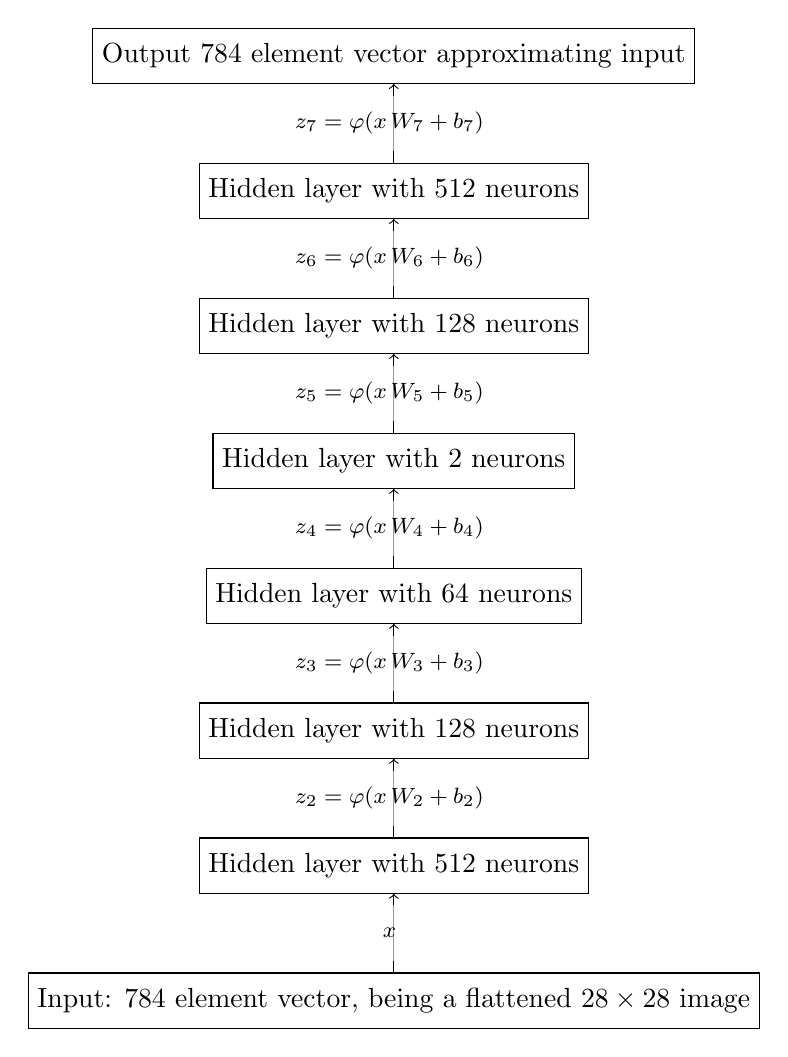
\begin{tikzpicture}[]

\node(L0)[layer]{Input: 784 element vector, being a flattened $28 \times 28$ image};

\foreach \i/\y[count=\j from 0] in {1/512, 2/128, 3/64, 4/2, 5/128, 6/512, 7/784}{
	\node(L\i)[layer, above= of L\j] {
		\ifthenelse{\j=6}{Output 784 element vector approximating input}%
		{Hidden layer with $\y$ neurons}%
	};
%
	\draw[->] (L\j) edge  node[labe]{
		\ifthenelse{\j = 0}{$x$}{$z_\i=\varphi(x\,W_\i+b_\i)$}
	}(L\i);	
}

%
\end{tikzpicture}

\end{document}}
\end{figure}


In this particular network $\varphi$ is a leaky RELU6 unit.
\asidefig[The Leaky ReLU6 function. The leak level on this plot is exaggerated for purposes of visualisation.]{
	\begin{tikzpicture}
	\begin{axis}[sideplot,  xtick={-6, 0,6}, ytick={-3, 0,3,6}, enlarge y limits={abs=2}]
	\addplot+[equ] {max(0.05*x, min(1.05*x, 0.05*x + 6))};
	\end{axis}
	\end{tikzpicture}
}
\begin{equation}
\varphi(z)=\begin{cases}
    0.01z+6 & 6<z \\
	1.01z & 0 \le z \le 6 \\
	0.01z & z < 0
\end{cases}
\end{equation}

The reason for this is that a sigmoidal unit does not perform well in a deep network because of the gradient-vanishing/exploding effects.
The effect of this to be that only the bias information of the final layer mattered -- effectively making all outputs just the average of all inputs.
The normal solution to this in deep networks is ReLU or ReLU6 units.

However, a ReLU, or ReLU6 unit is not ideal either,
as these units turn-off, and can not turn back on again.
If one of the just 2 neurons in the code layer turn-off then they can not turn back on again -- thus forcing it down to just one neuron, or none if that neural also dies.
In trialling this network structure, this was found to occur quiet very often.

The solution was to add a ``leak'' to the unit.
A small constant gradient even in the saturated position.
Making such a neuron possible, if difficult, to turn back on once turned off.
With this change the network always produces quality results.
An example of the recreation of an input from the test set can be seen in 
 \Cref{fig-ae-recreation}. 
It can be seen that the blur suggests that the input is a 7 or 9 like shape -- that level of information survived being squeezed through the bottleneck.


\asidefig[Recreation of an input from the MNIST test set. Input is on the left, output is on the right. 	{\label{fig-ae-recreation}}]{\includegraphics[scale=0.30]{figs/chapterintromachinelearning/recreation}}


More significantly, a sampling of the code layer is visually shown in \Cref{mnist-encoding}.
In this image, the positions on the X and Y axis of the input images, are given by the values on the coded layer said images correspond to.
It can be seen the the code is capturing key information about the appearance.
The 0s appear near to the similarly rounded 6s,
the 8s near the 3s, etc.
In particular the 1s are arrayed according to the their slope.
The autoencoder has captured very useful information about the inputs, that would be hard to define with any hand-written feature extractor.

It is this property of networks, to implicitly discover and define the most important latent variables and relationships to the task at hand that also makes the valuable for natural language processing.


\end{document}